
%% bare_conf.tex
%% V1.3
%% 2007/01/11
%% by Michael Shell
%% See:
%% http://www.michaelshell.org/
%% for current contact information.
%%
%% This is a skeleton file demonstrating the use of IEEEtran.cls
%% (requires IEEEtran.cls version 1.7 or later) with an IEEE conference paper.
%%
%% Support sites:
%% http://www.michaelshell.org/tex/ieeetran/
%% http://www.ctan.org/tex-archive/macros/latex/contrib/IEEEtran/
%% and
%% http://www.ieee.org/

%%*************************************************************************
%% Legal Notice:
%% This code is offered as-is without any warranty either expressed or
%% implied; without even the implied warranty of MERCHANTABILITY or
%% FITNESS FOR A PARTICULAR PURPOSE! 
%% User assumes all risk.
%% In no event shall IEEE or any contributor to this code be liable for
%% any damages or losses, including, but not limited to, incidental,
%% consequential, or any other damages, resulting from the use or misuse
%% of any information contained here.
%%
%% All comments are the opinions of their respective authors and are not
%% necessarily endorsed by the IEEE.
%%
%% This work is distributed under the LaTeX Project Public License (LPPL)
%% ( http://www.latex-project.org/ ) version 1.3, and may be freely used,
%% distributed and modified. A copy of the LPPL, version 1.3, is included
%% in the base LaTeX documentation of all distributions of LaTeX released
%% 2003/12/01 or later.
%% Retain all contribution notices and credits.
%% ** Modified files should be clearly indicated as such, including  **
%% ** renaming them and changing author support contact information. **
%%
%% File list of work: IEEEtran.cls, IEEEtran_HOWTO.pdf, bare_adv.tex,
%%                    bare_conf.tex, bare_jrnl.tex, bare_jrnl_compsoc.tex
%%*************************************************************************

% *** Authors should verify (and, if needed, correct) their LaTeX system  ***
% *** with the testflow diagnostic prior to trusting their LaTeX platform ***
% *** with production work. IEEE's font choices can trigger bugs that do  ***
% *** not appear when using other class files.                            ***
% The testflow support page is at:
% http://www.michaelshell.org/tex/testflow/



% Note that the a4paper option is mainly intended so that authors in
% countries using A4 can easily print to A4 and see how their papers will
% look in print - the typesetting of the document will not typically be
% affected with changes in paper size (but the bottom and side margins will).
% Use the testflow package mentioned above to verify correct handling of
% both paper sizes by the user's LaTeX system.
%
% Also note that the "draftcls" or "draftclsnofoot", not "draft", option
% should be used if it is desired that the figures are to be displayed in
% draft mode.
%
\documentclass[10pt, conference, compsocconf]{IEEEtran}
% Add the compsocconf option for Computer Society conferences.
%
% If IEEEtran.cls has not been installed into the LaTeX system files,
% manually specify the path to it like:
% \documentclass[conference]{../sty/IEEEtran}





% Some very useful LaTeX packages include:
% (uncomment the ones you want to load)


% *** MISC UTILITY PACKAGES ***
%
%\usepackage{ifpdf}
% Heiko Oberdiek's ifpdf.sty is very useful if you need conditional
% compilation based on whether the output is pdf or dvi.
% usage:
% \ifpdf
%   % pdf code
% \else
%   % dvi code
% \fi
% The latest version of ifpdf.sty can be obtained from:
% http://www.ctan.org/tex-archive/macros/latex/contrib/oberdiek/
% Also, note that IEEEtran.cls V1.7 and later provides a builtin
% \ifCLASSINFOpdf conditional that works the same way.
% When switching from latex to pdflatex and vice-versa, the compiler may
% have to be run twice to clear warning/error messages.






% *** CITATION PACKAGES ***
%
%\usepackage{cite}
% cite.sty was written by Donald Arseneau
% V1.6 and later of IEEEtran pre-defines the format of the cite.sty package
% \cite{} output to follow that of IEEE. Loading the cite package will
% result in citation numbers being automatically sorted and properly
% "compressed/ranged". e.g., [1], [9], [2], [7], [5], [6] without using
% cite.sty will become [1], [2], [5]--[7], [9] using cite.sty. cite.sty's
% \cite will automatically add leading space, if needed. Use cite.sty's
% noadjust option (cite.sty V3.8 and later) if you want to turn this off.
% cite.sty is already installed on most LaTeX systems. Be sure and use
% version 4.0 (2003-05-27) and later if using hyperref.sty. cite.sty does
% not currently provide for hyperlinked citations.
% The latest version can be obtained at:
% http://www.ctan.org/tex-archive/macros/latex/contrib/cite/
% The documentation is contained in the cite.sty file itself.






% *** GRAPHICS RELATED PACKAGES ***
%
\ifCLASSINFOpdf
   \usepackage[pdftex]{graphicx}
  % declare the path(s) where your graphic files are
   \graphicspath{{../figs/}}
  % and their extensions so you won't have to specify these with
  % every instance of \includegraphics
   \DeclareGraphicsExtensions{.pdf,.jpeg,.png}
\else
  % or other class option (dvipsone, dvipdf, if not using dvips). graphicx
  % will default to the driver specified in the system graphics.cfg if no
  % driver is specified.
   \usepackage[dvips]{graphicx}
  % declare the path(s) where your graphic files are
  % \graphicspath{{../eps/}}
  % and their extensions so you won't have to specify these with
  % every instance of \includegraphics
  % \DeclareGraphicsExtensions{.eps}
\fi
% graphicx was written by David Carlisle and Sebastian Rahtz. It is
% required if you want graphics, photos, etc. graphicx.sty is already
% installed on most LaTeX systems. The latest version and documentation can
% be obtained at: 
% http://www.ctan.org/tex-archive/macros/latex/required/graphics/
% Another good source of documentation is "Using Imported Graphics in
% LaTeX2e" by Keith Reckdahl which can be found as epslatex.ps or
% epslatex.pdf at: http://www.ctan.org/tex-archive/info/
%
% latex, and pdflatex in dvi mode, support graphics in encapsulated
% postscript (.eps) format. pdflatex in pdf mode supports graphics
% in .pdf, .jpeg, .png and .mps (metapost) formats. Users should ensure
% that all non-photo figures use a vector format (.eps, .pdf, .mps) and
% not a bitmapped formats (.jpeg, .png). IEEE frowns on bitmapped formats
% which can result in "jaggedy"/blurry rendering of lines and letters as
% well as large increases in file sizes.
%
% You can find documentation about the pdfTeX application at:
% http://www.tug.org/applications/pdftex





% *** MATH PACKAGES ***
%
\usepackage[cmex10]{amsmath}
% A popular package from the American Mathematical Society that provides
% many useful and powerful commands for dealing with mathematics. If using
% it, be sure to load this package with the cmex10 option to ensure that
% only type 1 fonts will utilized at all point sizes. Without this option,
% it is possible that some math symbols, particularly those within
% footnotes, will be rendered in bitmap form which will result in a
% document that can not be IEEE Xplore compliant!
%
% Also, note that the amsmath package sets \interdisplaylinepenalty to 10000
% thus preventing page breaks from occurring within multiline equations. Use:
%\interdisplaylinepenalty=2500
% after loading amsmath to restore such page breaks as IEEEtran.cls normally
% does. amsmath.sty is already installed on most LaTeX systems. The latest
% version and documentation can be obtained at:
% http://www.ctan.org/tex-archive/macros/latex/required/amslatex/math/





% *** SPECIALIZED LIST PACKAGES ***
%
%\usepackage{algorithmic}
\usepackage[ruled,vlined,commentsnumbered]{algorithm2e}
%\usepackage{algpseudocode}
% algorithmic.sty was written by Peter Williams and Rogerio Brito.
% This package provides an algorithmic environment fo describing algorithms.
% You can use the algorithmic environment in-text or within a figure
% environment to provide for a floating algorithm. Do NOT use the algorithm
% floating environment provided by algorithm.sty (by the same authors) or
% algorithm2e.sty (by Christophe Fiorio) as IEEE does not use dedicated
% algorithm float types and packages that provide these will not provide
% correct IEEE style captions. The latest version and documentation of
% algorithmic.sty can be obtained at:
% http://www.ctan.org/tex-archive/macros/latex/contrib/algorithms/
% There is also a support site at:
% http://algorithms.berlios.de/index.html
% Also of interest may be the (relatively newer and more customizable)
% algorithmicx.sty package by Szasz Janos:
% http://www.ctan.org/tex-archive/macros/latex/contrib/algorithmicx/




% *** ALIGNMENT PACKAGES ***
%
%\usepackage{array}
% Frank Mittelbach's and David Carlisle's array.sty patches and improves
% the standard LaTeX2e array and tabular environments to provide better
% appearance and additional user controls. As the default LaTeX2e table
% generation code is lacking to the point of almost being broken with
% respect to the quality of the end results, all users are strongly
% advised to use an enhanced (at the very least that provided by array.sty)
% set of table tools. array.sty is already installed on most systems. The
% latest version and documentation can be obtained at:
% http://www.ctan.org/tex-archive/macros/latex/required/tools/


%\usepackage{mdwmath}
%\usepackage{mdwtab}
% Also highly recommended is Mark Wooding's extremely powerful MDW tools,
% especially mdwmath.sty and mdwtab.sty which are used to format equations
% and tables, respectively. The MDWtools set is already installed on most
% LaTeX systems. The lastest version and documentation is available at:
% http://www.ctan.org/tex-archive/macros/latex/contrib/mdwtools/


% IEEEtran contains the IEEEeqnarray family of commands that can be used to
% generate multiline equations as well as matrices, tables, etc., of high
% quality.


%\usepackage{eqparbox}
% Also of notable interest is Scott Pakin's eqparbox package for creating
% (automatically sized) equal width boxes - aka "natural width parboxes".
% Available at:
% http://www.ctan.org/tex-archive/macros/latex/contrib/eqparbox/





% *** SUBFIGURE PACKAGES ***
%\usepackage[tight,footnotesize]{subfigure}
% subfigure.sty was written by Steven Douglas Cochran. This package makes it
% easy to put subfigures in your figures. e.g., "Figure 1a and 1b". For IEEE
% work, it is a good idea to load it with the tight package option to reduce
% the amount of white space around the subfigures. subfigure.sty is already
% installed on most LaTeX systems. The latest version and documentation can
% be obtained at:
% http://www.ctan.org/tex-archive/obsolete/macros/latex/contrib/subfigure/
% subfigure.sty has been superceeded by subfig.sty.



%\usepackage[caption=false]{caption}
%\usepackage[font=footnotesize]{subfig}
% subfig.sty, also written by Steven Douglas Cochran, is the modern
% replacement for subfigure.sty. However, subfig.sty requires and
% automatically loads Axel Sommerfeldt's caption.sty which will override
% IEEEtran.cls handling of captions and this will result in nonIEEE style
% figure/table captions. To prevent this problem, be sure and preload
% caption.sty with its "caption=false" package option. This is will preserve
% IEEEtran.cls handing of captions. Version 1.3 (2005/06/28) and later 
% (recommended due to many improvements over 1.2) of subfig.sty supports
% the caption=false option directly:
%\usepackage[caption=false,font=footnotesize]{subfig}
%
% The latest version and documentation can be obtained at:
% http://www.ctan.org/tex-archive/macros/latex/contrib/subfig/
% The latest version and documentation of caption.sty can be obtained at:
% http://www.ctan.org/tex-archive/macros/latex/contrib/caption/




% *** FLOAT PACKAGES ***
%
%\usepackage{fixltx2e}
% fixltx2e, the successor to the earlier fix2col.sty, was written by
% Frank Mittelbach and David Carlisle. This package corrects a few problems
% in the LaTeX2e kernel, the most notable of which is that in current
% LaTeX2e releases, the ordering of single and double column floats is not
% guaranteed to be preserved. Thus, an unpatched LaTeX2e can allow a
% single column figure to be placed prior to an earlier double column
% figure. The latest version and documentation can be found at:
% http://www.ctan.org/tex-archive/macros/latex/base/



%\usepackage{stfloats}
% stfloats.sty was written by Sigitas Tolusis. This package gives LaTeX2e
% the ability to do double column floats at the bottom of the page as well
% as the top. (e.g., "\begin{figure*}[!b]" is not normally possible in
% LaTeX2e). It also provides a command:
%\fnbelowfloat
% to enable the placement of footnotes below bottom floats (the standard
% LaTeX2e kernel puts them above bottom floats). This is an invasive package
% which rewrites many portions of the LaTeX2e float routines. It may not work
% with other packages that modify the LaTeX2e float routines. The latest
% version and documentation can be obtained at:
% http://www.ctan.org/tex-archive/macros/latex/contrib/sttools/
% Documentation is contained in the stfloats.sty comments as well as in the
% presfull.pdf file. Do not use the stfloats baselinefloat ability as IEEE
% does not allow \baselineskip to stretch. Authors submitting work to the
% IEEE should note that IEEE rarely uses double column equations and
% that authors should try to avoid such use. Do not be tempted to use the
% cuted.sty or midfloat.sty packages (also by Sigitas Tolusis) as IEEE does
% not format its papers in such ways.





% *** PDF, URL AND HYPERLINK PACKAGES ***
%
%\usepackage{url}
% url.sty was written by Donald Arseneau. It provides better support for
% handling and breaking URLs. url.sty is already installed on most LaTeX
% systems. The latest version can be obtained at:
% http://www.ctan.org/tex-archive/macros/latex/contrib/misc/
% Read the url.sty source comments for usage information. Basically,
% \url{my_url_here}.





% *** Do not adjust lengths that control margins, column widths, etc. ***
% *** Do not use packages that alter fonts (such as pslatex).         ***
% There should be no need to do such things with IEEEtran.cls V1.6 and later.
% (Unless specifically asked to do so by the journal or conference you plan
% to submit to, of course. )


% correct bad hyphenation here
\hyphenation{op-tical net-works semi-conduc-tor}


\begin{document}
%
% paper title
% can use linebreaks \\ within to get better formatting as desired
\title{Large Data and Computation in a Hazard Map Workflow Using Hadoop and Multiscale Emulator Methods}


% author names and affiliations
% use a multiple column layout for up to two different
% affiliations

%\author{\IEEEauthorblockN{E.~Ramona Stefanescu}
%\IEEEauthorblockA{Dept. of Mech. Eng.\\
%University at Buffalo\\
%New York, USA\\
%ers32@buffalo.edu}
%\and
%\IEEEauthorblockN{Shivaswamy Rohit}
%\IEEEauthorblockA{Dept. of Mech. Eng.\\
%University at Buffalo\\
%New York, USA\\
%shivaswa@buffalo.edu}
%\and
%\IEEEauthorblockN{Abani~K. Patra}
%\IEEEauthorblockA{Dept. of Mech. Eng.\\
%University at Buffalo\\
%New York, USA\\
%abani@buffalo.edu}
%}
% conference papers do not typically use \thanks and this command
% is locked out in conference mode. If really needed, such as for
% the acknowledgment of grants, issue a \IEEEoverridecommandlockouts
% after \documentclass

% for over three affiliations, or if they all won't fit within the width
% of the page, use this alternative format:
% 
\author{\IEEEauthorblockN{E.~Ramona Stefanescu\IEEEauthorrefmark{1},
Shivaswamy Rohit\IEEEauthorrefmark{1} and
Abani K. Patra\IEEEauthorrefmark{1}}
\IEEEauthorblockA{\IEEEauthorrefmark{1}Department of Mechanical and Aerospace Engineering \\
University at Buffalo,
Buffalo, New York 14260--4400\\ Email: abani@buffalo.edu}}
%\IEEEauthorblockA{\IEEEauthorrefmark{2}Twentieth Century Fox, Springfield, USA\\
%Email: homer@thesimpsons.com}}




% use for special paper notices
%\IEEEspecialpapernotice{(Invited Paper)}




% make the title area
\maketitle


\begin{abstract}
Three main processes are required in order to construct a simulation based probabilistic hazard map for volcanic 
debris: a) a good physical model, i.e. a simulator, with error control; b) an approach to uncertainty 
quantification usually involving an ensemble of simulator runs and an easily sampled  surrogate model; c) a multiscale process to analyze the simulator 
output into a map of the probability that some hazard criteria will be met.
The above processes lead to large amount of data and  CPU  intensive computing. This work advances state 
of the art in the last area, by deploying a novel programming model; and also by using a hierarchical approach in creating a fast surrogate of the simulator.
Handling the huge amount of data and computing is a primary concern in constructing a hazard map on distributed memory platforms. We describe a framework that we built using 
Hadoop to parallelize the data and compute intensive operations. We make use of Hadoop�s MapReduce framework 
to improve the speed of hazard map creation.
\end{abstract}

\begin{IEEEkeywords}
Uncertainty Quantification; Multiscale Emulator; Hadoop;

\end{IEEEkeywords}


% For peer review papers, you can put extra information on the cover
% page as needed:
% \ifCLASSOPTIONpeerreview
% \begin{center} \bfseries EDICS Category: 3-BBND \end{center}
% \fi
%
% For peerreview papers, this IEEEtran command inserts a page break and
% creates the second title. It will be ignored for other modes.
\IEEEpeerreviewmaketitle



\section{Introduction}
For the purpose of this paper, we will assume that a suitable physical model of geophysical mass flow is available 
(TITAN2D).  Any simulator will naturally require values for certain input parameters. If the input values for a 
future event of interest were known exactly, then a hazard map could be generated from a single simulation 
evaluated at those inputs. Since we lack perfect knowledge of the future, it is necessary to examine flow behavior
over a range of inputs. While there are some sampling methods, such as Monte Carlo, that are \textit{nominally independent}
of the number of dimensions, there are far too expensive to use to create a feasible hazard map. 
The solution we came up to this problem can be summarized as:
\begin{itemize}
\item Running a \textit{relatively} small number of simulations (a few hundred to a few thousand) followed by
\item Constructing a meta-model (a model of the simulator) to act as a fast surrogate for the expensive simulator, and then
\item Generating the hazard map from the fast surrogate. 
\end{itemize}
In this work we introduce a multi-resolution scheme for an emulator construction on a high-dimensional parameter space. The 
proposed scheme overcomes some limitations of the 
parameter selection in the Bayesian emulator, which always  involves  repeated  inversion  of  error ``correlation  matrix",  $R$. 
The requirement  of  matrix  inversion  restricts  emulators  to  small  amounts  of  data mostly because for ``large" $N$:  $R$ is 
poorly conditioned and cost  of  inverting  matrix  is  $\mathcal{O}(N^3)$ operations.
Our scheme is based on mutual distances between data points and on a continuous extension of Gaussian functions. It uses a corse-to-fine hierarchy of the multi-resolution decomposition of a Gaussian kernel.
It generates a sequence of approximations at the given function on the data, as well as their extensions to any
newly-arrived data point. The subsampling is done by interpolative decomposition of the associated Gaussian kernel matrix in each scale in the hierarchical procedure. In this way a well-conditioned basis is identified and used in the extension/ extrapolation process. 


\section{Computational challenages}
A hazard map, as stated here, is a predictive map for a region  
which provides a probabilistic measure of
a hazard (e.g. geophysical flow reaching certain depths that can be considered hazardous/critical).
Simple uncertainty quantification using a Monte Carlo approach for generating such hazard maps will require $O(10^6)$ such simulations 
-- beyond current computational capabilities.
Since each flow simulation generates upwards of 2GB of data, a full ensemble with 2048 simulations generates almost 600GB of data which 
we have to then use to construct emulators. The computational difficulties include managing and accessing select entities 
from the large data and of processing it using compute intensive operations. Our approach to addressing these difficulties 
is to decouple the data mining and computationally intensive tasks through carefully crated workflows. 
We thus, employ the popular open source version of the Map-Reduce model, namely Hadoop, both in conjunction with a high performance cluster.
Problems involved in data extraction, movement over the 
network, and replication are addressed. The proposed computational methodologies also allow us to greatly improve the resolution of the 
developed hazard maps by using a hierarchical approach (rather than the simpler tessellation based localization used earlier \cite{keith}) 
allowing access to more data in the inference process and hence developing a more accurate localization of the covariance used in the hazard 
map construction.

\section{Multiscale emulator}
In the analysis of large scale simulations of complex dynamical systems, where the notion of time evolution comes into play, important problems 
are the identification of variables that capture the time evolution of the system. Traditionally, creating hazard maps has required detailed knowledge 
of past events which has been recorded in the volcano's geologic record. Knowledge of this history is frequently incomplete or even entirely unavailable.
Our goal is to produce a map showing the probability that each East-North point has of being inundated by a volcanic landslide with a flow-depth greater than a critical threshold from a collection of simulator runs whose parameters are drawn from a distribution that represents a volcanologist's best guess of the range of possible scenarios. We consider a study case for Soufri\`ere Hills, Montserrat, for which ranges of the flow volume, bed friction, internal friction and direction are available.
The 4-dimensional input parameter space is sampled using a simple space filling design like Latin Hypercube Design (LHD) to obtain 2048 sets of input. Simulations are performed at each sample point using the TITAN2D model to generate a map of maximum pile height, $h_{max}(\textbf{x})$ as function of position.
If we plot the maximum pile height at a specific location in space for each sample point we can easily observe the binning introduced by the LHD sampling (Fig.~\ref{fig_lhs} - blue dots). In LHD, each random direction (random variable or input) is divide into $N_{bin}$ bins of equal probability and one random value is selected in each bin \cite{mckay1979comparison}. 
\begin{figure}
\begin{center}
%\resizebox*{15cm}{!}{\includegraphics{net_flow.pdf}}
\resizebox*{9cm}{!}{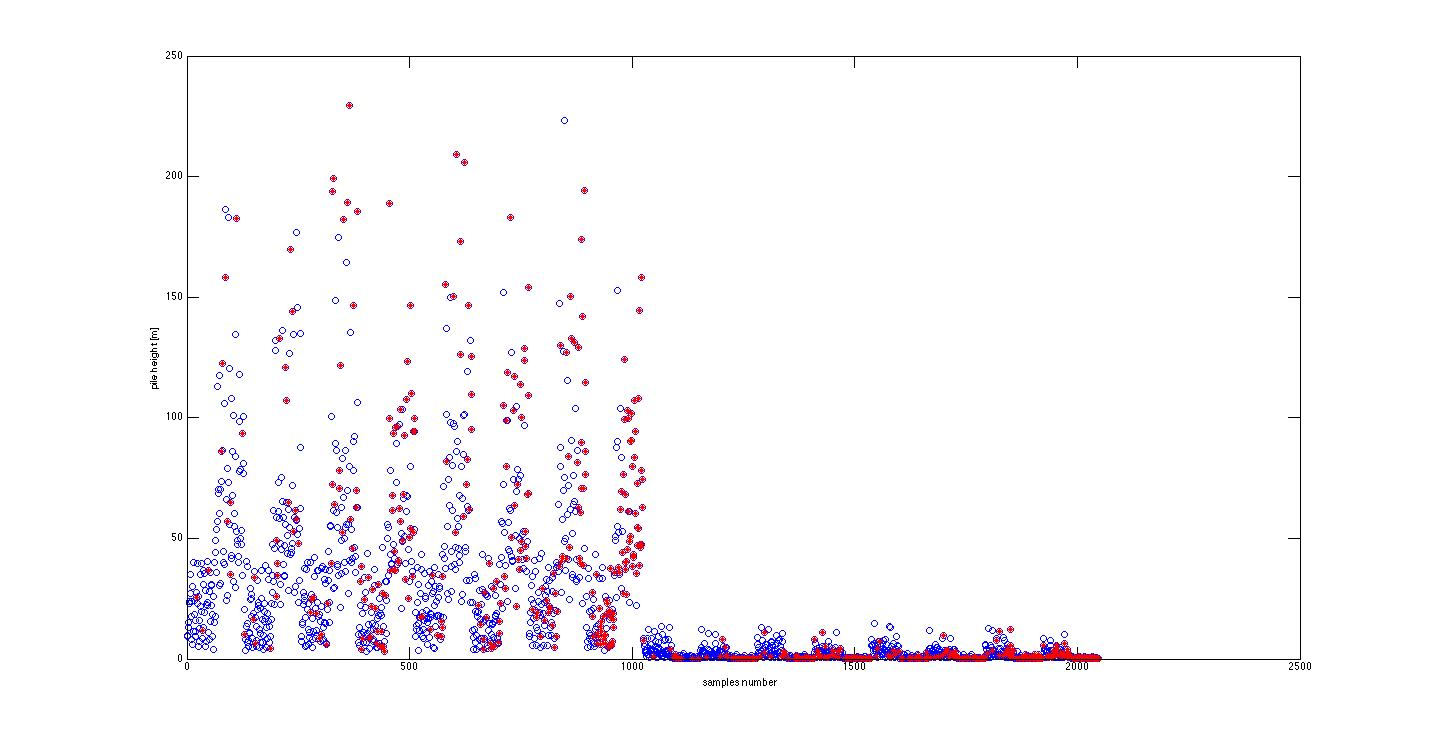
\includegraphics{lhs_hmax.jpg}}
\vspace{-30pt}
\caption{\label{fig_lhs} Blue dots represent the maximum pile heigh at a selected location for each LHD sample point, the red starts represent the multiscale data samples.}
\end{center}
\end{figure}
By performing a multiscale data sampling we identify a well-conditioned basis of a low rank Gaussian kernel matrix, used in identifying scattered data sampling (Fig.~\ref{fig_lhs} - red stars). Using the obtained sample data, $h_{max}$ is evaluated at re-sample points.

Typical usage involves evaluating the fast surrogate at hundreds of thousands or millions of re-sample input points. The number of samples needed to generate the fast surrogate are exponential in the number of dimensions. This effectively limits its application to when there are three or fewer uncertain dimensions. This implies that we need to change the representation of the 2048 data sets, into a low-dimensional that describe the data in a faithful manner. In order to achieve this goal, we use a technique that relies on graph-based algorithms. Weighted graphs are employed to represent the ``geometry" based on the local similarity or interaction between the data points. Since each of the data sample is represented by a collection of numerical attributes, the condition of two nodes to be connected is based on the proximity of the corresponding data points in the feature space.

A graph $G=(V,E)$ is characterized by a set of vertices $V=\{1,\dots,m\}$ and a set of edges $E=\{e_{ij}|i,j \in V\}$.
Let $A=[a_{ij}]$ be the $m\times m$ adjacency matrix such that $a_{ij}$ represents the weight of edge $e_{ij}$. If there is no edge between vertices $i$ and $j$ then $a_{ij}=0$.
Clustering the vertices $V$ into $c$ disjoints sets $V_1, \dots, V_c$ with $m_i=|V_i|$, the adjacency matrix will have
the following form:
\begin{equation}
A_{m,n} =
 \begin{bmatrix}
  A_{11}  & \cdots & A_{1c} \\
  A_{2,1} & \cdots & A_{2,n} \\
  \vdots  & \ddots & \vdots  \\
  A_{c1}  & \cdots & A_{c,c}
 \end{bmatrix}
\end{equation}
where each diagonal block $A_{ii}, i=1,\dots,c$, is an $m_i \times m_i$ matrix that can be considered as a local
adjacency matrix for cluster $i$. The off-diagonal $m_i \times m_j$ blocks $A_{ij}$ with $i \neq j$, contain the
set of edges between vertices belonging to different clusters.

In a perfectly clusterable graphs, the off-diagonal blocks will not contain any edges, thus yielding $A_{ij}=0$,
and the graph will consist of $c$ disconnected components. In a realistic scenario, with a graph forming good clusters
most of the edges will be contained within the diagonal blocks $A_{ii}$, while the off-diagonal blocks $A_{ij}$ will
contain only a few edges.
The decay in the $A$'s spectrum is a measure of the connectivity of the points in the graph.
\begin{itemize}
\item One extreme case corresponds to the graph where all the all the nodes are disconnected. This leads to
$A$ being equal to the identity operator and thus to a flat spectrum.
\item Another case is the graph where all the nodes are connected to all the other nodes weights equal to
$1$. In this case, $A$ has one eigenvalue equal to 1, and all other eigenvalues are equal to 0 (we obtain the
fastest decay possible for the a diffusion operator).
\item Usually the spectrum of the heat kernel decays smoothly. 
\end{itemize}

Many dimensionality reduction methods involve a spectral decomposition of large matrices, whose dimensions are proportional to the size of the data, has high computational cost. The $n$ observations
${f_1,f_2,\dots, f_3}$ are considered the data points.
When the covariance of the data points is unknown, an artificial function has to be chose. A Gaussian covariance is a popular choice:
\begin{align}
g_{\epsilon}(x,x') = exp(- \parallel x-x' \parallel ^ 2 / \epsilon)
\end{align}
where $\parallel\dots\parallel$ constitutes a metric on the space (Euclidean distance in our case). The corresponding covariance (affinities) is
\begin{align}
(G_{\epsilon})=g_{\epsilon}(x_i,x_j), \; i,j=1,2,\dots,n.
\end{align}
The combination of clustering and low rank approximation gives a better approximation of the 
original graph. A standard low rank computation is likely to only extract information from the
largest or a few dominant clusters. 
The $Nystr\ddot{o}m$ method, vastly used for out-of-sample extension has three significant disadvantages: (a) Diagonalization of $G$ costs $\mathcal{O}(n^3)$ operations; (b) $G$ may be 
ill-conditioned due to fast decay of its spectrum, and (c) it is unclear how to choose the length parameter $\epsilon$ since the output is sensitive to the choice of $\epsilon$.
To overcome these limitations a multiscale approach is used: a sequence of Gaussian kernel matrices $G_s, s=0,1, \dots$, whose entries are $(G_{\epsilon})=g_{\epsilon}(x_i,x_j)$, where 
$\epsilon_s$ is a positive monotonic decreasing function of $s$, which tends to zero as the scale parameter $s$ tends to infinity (i.e. $\epsilon_s=2^{-s}$, $s=0,1,\dots$.). 

By the application of a randomized interpolative decomposition(ID) to $G_s$, a well-conditioned basis is identified for it numerical range. In each scale $f$ is decomposed into a sum of its 
projections on this basis and it is extended as $\bar{f}_{*} = G_{*}G^{-1}f$. In addition, selection of the proper columns in $G_s$ is equivalent to data sampling of the associated data points.

The method requires no grid. It automatically generates a sequence of adaptive grids according to the data distribution. It is based on the mutual distances between the data points and on a continuous 
extension of Gaussian functions. In addition, most of the costly computations are done just once during the process, independently of the number of the extended data points since they depend only in the data and on the given function. 

\begin{algorithm}
\SetAlgoLined
 \KwData{A data set $D=\{x_1,\dots,x_n\} \in \mathcal{R}^d$ (based on LHS design) }
 \KwResult{A function $f= [f_1,\dots,f_n]^T$}
 \While {$i \le n$}{
  Run TITAN2D simulation for each $x_i$. \\
  Use a downsample algorithm  $\rightarrow$ $N$ downsample points.\\
  For each $N$ generate an $f$ based on maximum height and apply the response surface calculation algorithm.\\
  Perform multiscale d
  
  
  }
\caption{Initial setup}
\end{algorithm}
  
\begin{algorithm}
 \SetAlgoLined
 \KwData{A data set $D=\{x_1,\dots,x_n\} \in \mathcal{R}^d$, $T>0$, a new data point $x_{*}\in \mathcal{R}^d$, a function $f= [f_1,\dots,f_n]^T$ to be
 extended and an error parameter $err \ge 0$. }
 \KwResult{An approximation $F=[F_1,\dots,F_n]^T$ of $f$ on $D$ and its extension $F_{*}$ to $x_{*}$ }
 Set the scale parameter $s=0$, $F^{(-1)}=0\in \mathcal{R}^n$ and $ F_{*}^{(-1)}=0$.\\
 \While{$\parallel f -F^{(-1)} \parallel > err$ }{
  Form the Gaussian kernel $G^{(s)}$on $D$ with $\epsilon_s=\frac{T}{2^s}$\;
  Estimate numerical rank $l^{(s)}$ of $G^{(s)}$\;
  Generate $A$ whose entries are i.i.d Gaussian random variables of zero mean and unit variance: $W=AG^{(s)}$\;
  Apply pivoted QR on $W$ $\rightarrow$ $WP_R=QR$\;
  Split R and Q st. \[
\left[
\begin{array}{c|c}
R_{11} & R_{12} \\
\hline
0 & R_{22}\\
\end{array}
\right]
\]
 and [ Q1 $\mid$ Q2] \;
    $S=Q_1R_{11}$ \;
    Columns of $S$ constitute a subset of of the columns of $W$. The corresponding columns of $G^{(s)}$ are collected into a matrix $B$,
    so that the column of $j$th column of $B^{(s)}$ is the $i_j$th column of $A$. The sampled dataset is $D_s$.\;
    Calculate the pseudo-inverse $(B^{(s)})^{\dagger}$ of $B^{(s)}$.\;
    Calculate the coordinates vector of the orthogonal projection of $f^{(s)}$ on the range of $B^{(s)}$ in the basis of $B^{(s)}$'s 
    columns $c=(B^{(s)})^{\dagger}f$\;
    Calculate the orthogonal projection of $f$ on the columns of $B^{(s)}$, $f^{(s)}=B^{(s)}c$\;
    Form the matrix $G^{(s)}_{*}=[g_{\epsilon}(x_*,x_{s_1}) \dots g_{\epsilon}(x_*,x_{s_{l^{(s)}}})]$\;
    Calculate the extension $f^{(s)}_* = G_{*}c$\;
    Set $F^{(s)}=F^{(s-1)} + f^{(s)}$, $F_{*}^{(s-1)}+f_{*}^{(s)}$, s=s+1\;
 }
 \caption{Response surface calculation}
\end{algorithm}




\section{ Hazard Map Generation --  Data Management and Computing}\label{HMG}
The simulator naturally require values for certain
input parameters, such as a digital model of the terrain, the volume of the flow,
material properties, and other initial conditions (starting location of the flow and a preferred
initial direction).
To understand the complexity of the problem
we present an outline of steps involved in a usual process of Hazard map generation. \\

\begin{itemize}
\vspace{-0.2in}
\item {\bf Step 0}: The first step is to run the simulator at well chosen inputs. The input parameters
%sample the parameters, to construct the emulator.
%which include but are not limited to the initial volume of pile, 2 parameters of
%location, and the internal friction, 
are sampled using a simple space filling design like Latin Hypercube to obtain  2048 sets of input.
Multiprocessor Titan2D  simulations of these inputs  and post processing results in 
2 gigabytes(GB) of flowdata per sample in the form of flow height records. 
%The input parameters along with spatial co-ordinates of the flow account 
%for all the random variables considered to induce uncertainty in the system.
\item {\bf Step 1}: { The construction of the hazard map requires us to sample a tensor product of the input parameters and 2 space dimensions
which results in as many as 10$^{8}$ data points. Emulator construction on this very large set is unaffordable so a simple 
contouring and decimation strategy is used to create a smaller set on which we construct the emulator.
This 
downsampling is introduced to reduce their number to the order of 10$^{6}$. Furthermore, 
resamples from the generated emulator surface (for the final probability calculation) are also required to be generated and can be as many as $10^{10}$ in number.}

\item {\bf Step 2}: The size of the downsized  data set makes it computationally impossible to fit a single emulator using all the data 
at once, which warrants the need for piecewise emulator obtained by localizing the covariance. The
neighbor search used in identifying the regions for localization is thus an important pre-requisite for the functioning of the
emulator and requires both sample and resamples to be searched from among the samples for neighbors. Both neighbor search and downsampling
are highly data intensive tasks which require little computation but scanning of large datasets.

\begin{figure}
\begin{center}
%\resizebox*{15cm}{!}{\includegraphics{net_flow.pdf}}
\resizebox*{10cm}{!}{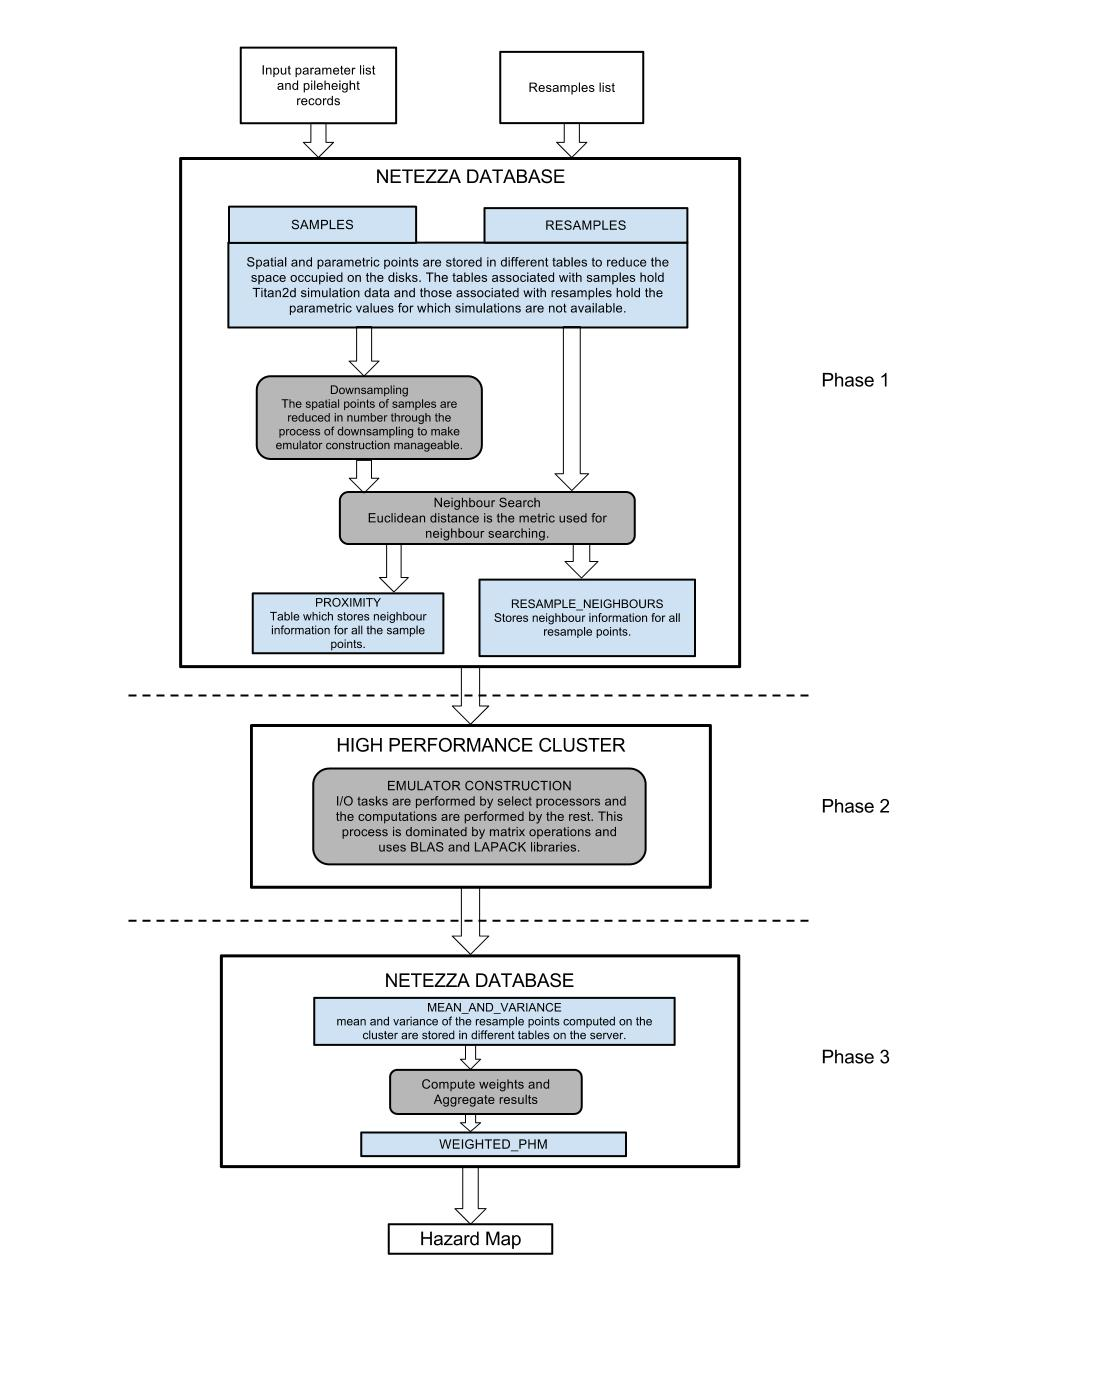
\includegraphics{Workflow2.jpg}}
\vspace{-40pt}
\caption{\label{fig2} Illustration of the integrated workflow using Netezza architecture.}%
\end{center}
\end{figure}

\begin{figure}
\begin{center}
%\resizebox*{15cm}{!}{\includegraphics{net_flow.pdf}}
\resizebox*{10cm}{!}{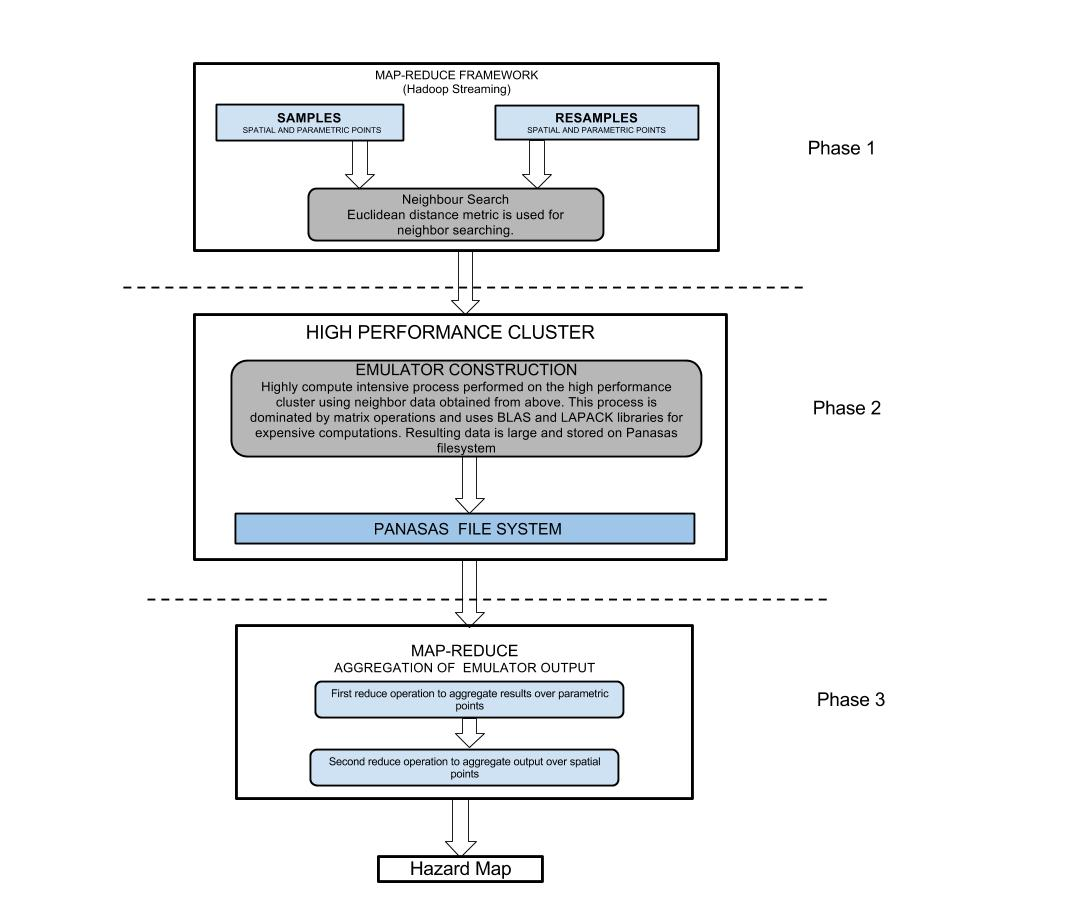
\includegraphics{Hadoop_Workflow.jpg}}
\vspace{-25pt}
\caption{\label{fig2} Illustration of the integrated workflow with Map-Reduce framework}
\end{center}
\end{figure}



\item {\bf Step 3}: Using neighborhood data, emulator is constructed about the sample points through an iterative process. 
The functioning of emulator can be understood from the following equations:
%by superimposing equations \ref{mean} and \ref{reg} which yields

%\begin{subequations}\label{mean1}
%\begin{equation}
%                                E(s(y)|s(x)) = g(y)\beta + {r(y)}^{T}{R}^{-1}\epsilon
%\end{equation}
%\begin{equation}
%                                Var[s(y)|s(x)] = {\sigma}^{2}(1 - {r(y)}^{T}{R}^{-1}r(y))
%\end{equation}
%\end{subequations}
%\begin{equation}
%                                r_{i}(y) = exp\left(-\sum_{n=1}^{N_{dim}} \theta_n(y_n-x_{i,n})^{2}\right)
%\end{equation}


g(y) being  the matrix of basis functions evaluated at the resample points and $\beta$ being the vector of least square co-efficients.
R is the matrix of the correlation functions at x such that R$_{i,j}$ = r$_{i}$(x$_{j}$) = r$_{j}$(y$_{i}$) and $\sigma$ is the variance.

%Equation \ref{mean1}(a) clearly indicates that the emulator is composed of a mean which is approximated using least square fit, and an error term
%which is modeled as a gaussian process with 

$s(x) = {\beta}G(x) + \hat{\epsilon}$ is the response function.

$\epsilon$ = s(x) - G(x)$\beta$ the true error evaluated at the sample points. 
$\theta$$_{n}$ is the
vector of hyper-parameters or roughness parameters and Ndim is the number of dimensions associated with the data set.


At each iteration 
$\beta$ and R$^{-1}$ are computed using updated values of hyper-parameters ($\theta$).
%The emulator is set up using the data from the neighborhood of the point about
%which it is constructed. A covariance matrix (required for the gaussian error model) has to be set up and its inverse computed through an iterative
%procedure to ascertain the correct correlation lengths.
Mean and variance are then evaluated for the resamples and adjusted using bayes
linear equations. Typically, a hazard map requires constructing a few million emulators.
The emulator construction dominated by O($n^{3}$) matrix operations is a highly compute intensive process but also embarrassingly
parallel.

\item {\bf Step 4}: In the last stage of hazard map construction, emulator output is aggregated using barycentric weights.
This involves scanning the dataset, computing the euclidean distance of the samples that influence a resample point, evaluating their weights
 and assembling the results.

\end{itemize}



\section{Integrated Workflow for data and compute intensive tasks}
%It is clear from section \ref{HMG} that 
There are three dominant phases of Hazard Map generation namely:
1) Downsampling and neighbor searching,
2) Emulator construction, and, 3)Aggregation of resulting data.
Our computational model based on a $\it{divide}$ $\it{and}$ $\it{conquer}$ strategy, segregates these phases and performs them on either Netezza
server or the high performance cluster depending on the computational requirements.

\subsection{Downsampling and neighbor search}
%Both downsampling and neighbor search are ideally suited to be performed on the Netezza database.
Both downsampling and neighbor search are ideally suited for distributed systems.
For multidimensional dataset, such as ours, operations like neighbor search are afflicted with the $\textit{curse of
dimensionality}$. Several tree and clustering based methods have been proposed but most converge to sequential search for higher dimensions
and/or are difficult to implement. Neighbor search operation 
on a distributed environment like Netezza server or on a cluster through Map-Reduce
implementation like Hadoop allows for a much simpler algorithm and adapts to large datasets.
Downsampling and Neighbor search on the Netezza system were easily accomplished because of its massively parallel architecture.
%Downsampling on the Netezza system required a single query applied to the entire dataset of pileheight records which
%selects points at regular intervals on the grid. 
%Previous implementation of this on HPC platforms were significantly complex \cite{keith}.
Netezza's high performance stems from filtering data close to disk and from its MPP architecture. Since a significant amount of data
movement is curtailed through the use of FPGA filtering, we abstained from using complex algorithms in favor of brute force
techniques. All Netezza based implementations were in plain SQL which ensured parallelism and high performance. 

We also tested same operations on the high performance cluster using python scripts, relying on Hadoop Streaming API for 
task distribution and scheduling. 
In a distributed environment the  underlying algorithm for neighbor search remains essentially the same as the
one used on Netezza server. The mapper  computes the distances between two sets of data (X and Y) and prints out the result as key-value
pair, key being the indices of dataset X and value being the indices of dataset Y  and the euclidean distance. 
In the absence of a customized partitioner
same keys are guaranteed to be dispatched to the same reduce task. The reduce operation merely involves printing out the indices of set Y
against the keys obtained from set X. Hadoop based implementation as in the case with Netezza was simple and concise.

In both our implementations euclidean distance was the metric for neighbor search.
The parametric neighbor search was performed independent of spatial neighbor search by
separately treating the two sets of dimensions. 
Though the brute force method of neighbor search has a complexity of O($n^{2}$), it is well suited for distributed environment
owing to good scalability.
the Netezza
architecture is ideally suited for such methods.  The distance based neighbor search also made it possible to more
precisely define the region of neighborhood which could not have been achieved using tessellation based neighbor search. A notable advantage
of neighbor search on the database is that it can be easily extended to even higher dimensions without the need of any significant changes in
the implementation.\\

Database operations played a pivotal role in our computing model by making the cumbersome task of data-mining on the cluster a rather elegant
and transparent process. Netezza's datawarehousing capabilities ensured that all data could be stored at one place as opposed to having it
scattered across a
large number of flat files on the cluster. Using SQL, clean and concise codes could be written with provision for easily making changes.
Several hundreds of lines of MATLAB code were replaced with less than hundred SQL queries. Data warehousing capability and ``under the hood" data
movement offered an enormous respite from the MATLAB implementation on the cluster where data movement was achieved by reading and writing of a
large number ASCII files. Table \ref{tables} lists some of the tables that were generated on Netezza for one of the cases prior to emulator
construction. Tables with rows of the order of millions and even close to 2 billion in case of table $\small{PROXIMITY}$ were generated with
ease.



%\begin{comment}
%\begin{table*}
%\centering
%\caption{Some Typical Commands}
%\begin{tabular}{|c|c|c|} \hline
%%Command&A Number&Comments\\ \hline
%\bf{Table Name} & \bf{Number of rows} & \bf{Description}\\ 
%Titan & 149,207,040 & Pileheight and spatial co-ordinates of all the sample points.\\ \hline
%Downsampled &  4,054,229 & Points retained after downsampling.\\ \hline
%Samples\_Scaled & 2048 & Input parameters used for simulation.\\ \hline
%Resamples & 99,304 & Input parameters for which simulation data is not available.\\ \hline
%Uniq\_Coord & 10,068 & Indices of unique points on the grid pertaining to downsampled data.\\ \hline
%Proximity & 1,903,673,287 & neighbors of every downsampled point.\\ \hline
%Macro\_neighbor & 214054 & neighbors of input parameters.\\ \hline
%Phm\_neighbors & 226,691,049 & neighbors of spatial points of resamples\\ \hline
%Resample\_neighbors & 466858 & neighbors of input parameters of resamples from the samples.\\ \hline
%%\texttt{{\char'134}alignauthor} & 100& Author alignment\\ \hline
%%\texttt{{\char'134}numberofauthors}& 200& Author enumeration\\ \hline
%%\texttt{{\char'134}table}& 300 & For tables\\ \hline
%%\texttt{{\char'134}table*}& 400& For wider tables\\ \hline
%\end{tabular}
%\end{table*}
%\end{comment}






%With the data mining operations successfully accomplished, all the information required for emulator construction was available for immediate
%use in the form of tables on Netezza database.
% However, unlike the computations up to this point, the emulator construction is a
%computationally expensive process involving large number of matrix operations. 

%For a 
%By performing a few simple tests it was clear that Netezza was
%not well suited for emulator construction.
% Since the emulator construction is dominated by matrix operations 
%We attempted large number
%of matrix multiplication operations on Netezza using SQL and deduced that emulator construction on the database 
%would not be feasible under a reasonable time frame.
 %Table \ref{mat} %shows the time taken for performing multiplication on matrices of size 200x200. 
%Figure \ref{mulplot} shows an almost linear dependence between the number of matrix multiplication operations for square matrices of size
%200x200 and the time taken. An extrapolation of this data yields the time taken for 4 million operations at approximately 7 hours. In practice,
%linear dependence would not extend over such large number of operations owing to limited memory on S-blades. Also the number of matrix
%operations is much larger than 4 million.\\



%\subsection{Integrating Netezza with High Performance Cluster}
\subsection{Emulator Construction}
Unlike the data mining operations up to this point, the emulator construction is a computationally expensive process dominated by 
matrix operations. Though emulator conctruction is an embarrassingly parallel process and Netezza server boasts of massively 
parallel architecture, it was, for variety of reasons as we describe below,
appropriate to siphon data off
the database to an architecture that could meet the emulator's computational demands. First, complex algorithms can not be easily translated
into a declarative language like SQL. Second, the number of blades available in our systems put a limit on the available processors. Also the
explicit use of high performance libraries like \textit{blas} and \textit{lapack} was not possible. Another subtle aspect
about emulator which advocates against its construction on the database is that it requires small chunks of data, more precisely the
neighborhood data. Netezza is  more appropriate for scanning large datasets. We present here the steps taken and the challenges faced in 
integrating server to the cluster.

The high performance cluster and the Netezza system were connected using Netezza's
ODBC driver. Data transfer across the two frameworks was possible largely through the use of named pipes. On linux systems a
named pipe is a type of file - FIFO file (FIFO being the acronym for First In First Out). A named pipe does not store or buffer data and
hence does not occupy storage space on the filesystem.\\
Loading data from cluster to Netezza was achieved through the \textit{nzload} feature. The \textit{nzload} command is a SQL CLI client
application which in conjunction with named pipes that makes it possible to load data 
to Netezza server from any remote client\cite{data_load}. 
%Use of nzload together with named
%pipes greatly simplified transfer of data. The nzload command makes direct insertions to the target table, and the transaction is committed on
%closing the pipe. Multiple instances of nzload, can simultaneously load data on the server in  parallel.\\

\begin{figure}
\begin{center}
\resizebox*{8cm}{!}{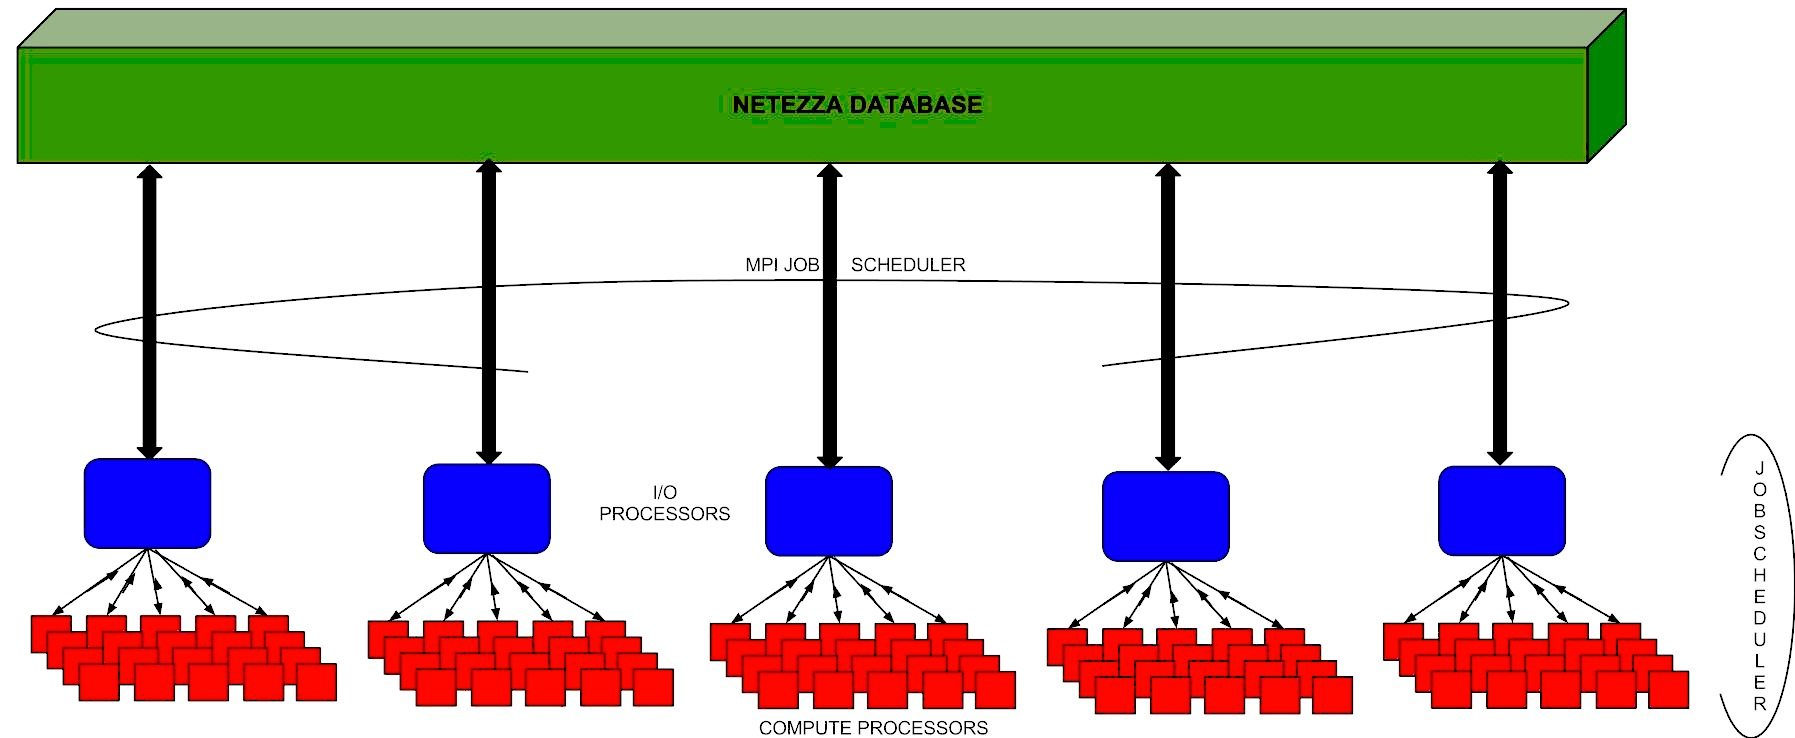
\includegraphics{cluster.jpg}}
\caption{\label{fig2} Schematic representation of integration of Netezza with high performance cluster}%
\end{center}
\end{figure}


\begin{figure*}
\begin{center}
\resizebox*{7cm}{!}{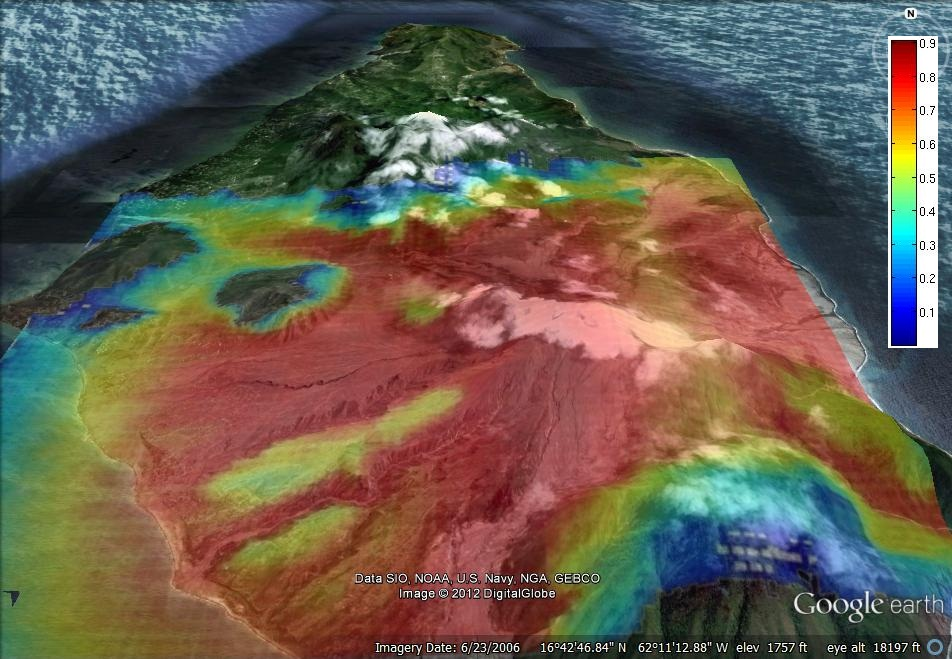
\includegraphics{new_map_colorbar.jpg}} %
\resizebox*{7.4cm}{!}{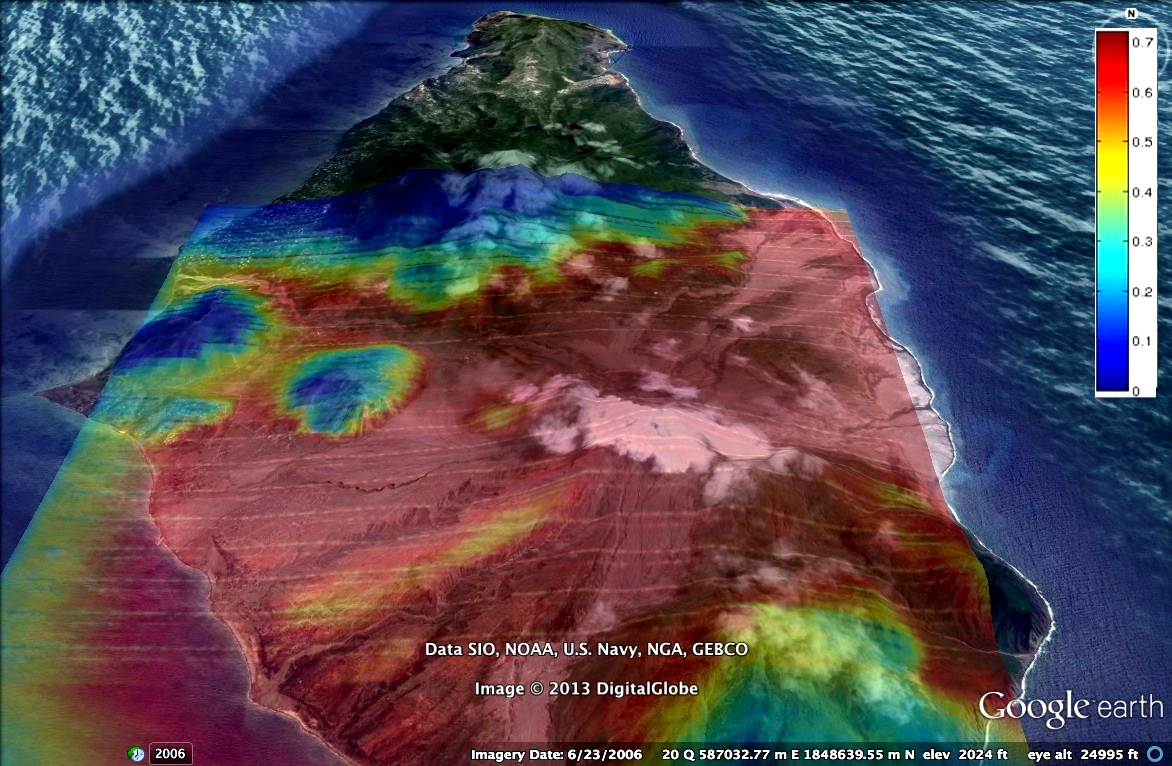
\includegraphics{Hadoop_map.jpg}}%
\caption {Figure shows the probabilistic hazard maps for the island of Montserrat in the Caribbean for flow exceeding 0.2m of depth.
One on left was generated using Netezza database based model and the one on right using Hadoop API} \label{map2}
\label{maps}
\end{center}
\end{figure*}


Emulator construction requires that each processor request the server for its share of data. Large number of concurrent I/O requests by nodes
on the grid can result in I/O bottlenecks and processors starving for data. Such problems have been addressed in the past and techniques such
as collective I/O\cite{cite4,kotz} and I/O forwarding\cite{cite5} have been proposed. I/O forwarding mitigates this problem by passing the I/O
requests of the all the nodes to only a select number of nodes called as I/O nodes. We adopted this method for our computing model with some
modifications.\\
A few processors on the high performance cluster are identified as the I/O processors and the rest as compute processors. All the processors
are assigned a group, with each group having one I/O processor and several compute processors. Each group operates independent of the other
with I/O processors responsible for performing all I/O operations on behalf of the compute processors of their respective groups. I/O
processors alone communicate with the Netezza server and any transfer of data occurs through named pipes. Multiple small requests are avoided
and data is invariably transferred in bulk. I/O processors extract data from Netezza, disseminate it across the compute processors and deliver
the data gathered from the compute processors back to the Netezza database. I/O processors of every group draw the neighborhood data of all
the downsampled points corresponding to the pileheight simulation number assigned to them from sever, and store it in their data structures.
Each compute processor based on the data received from the I/O processor of its group builds an emulator. The mean and variance data of the
resample points, computed at the end is sent over the network to I/O processor.\\
The operations on the cluster are parallelized using MPI (Message Passing Interface). Data is transferred between the I/O and compute processors
over the network using MPI protocols. An MPI job scheduler allows compute processors to notify the I/O processors about the status of their
completion. When a compute processor finishes constructing emulator about a sample point, it prompts the I/O processor. The I/O processor
responds by sending neighborhood data for the next point. The compute processors do not communicate among themselves and are self sufficient
with the data received from the I/O processor. The mean and variance information received from the compute processors is allowed to accumulate
with I/O processors and dispatched to the Netezza server at regular intervals. Another layer of MPI job-scheduler is responsible for
co-ordination between the various groups of processors. A lone processor which holds the metadata maintains communication with the groups and
assigns each group a simulation number to work on. Additionally it also prompts Netezza database to ``generate statistics" after each load
session.

Though we succeeded in integrating server with the cluster and in transferring data over the network, this implementation has apparent
shortcomings. Firstly offloading compute intensive tasks from server to cluster defeats the objective of minimizing large data movement.
Secondly only a small number of ports can be kept working between the two, to transfer data. Thus, though Netezza can easily house much
more data, extracting it to more nodes on cluster is not feasible. It is thus clear that compute intensive tasks like emulator construction
expose the vulnerabilities of even a specialized hardware like Netezza database. For the above mentioned reasons and also because of the 
complexity of implementation,  we attempted to test the above model with Hadoop in place of Netezza. Hadoop provides a convenient alternative
because it does not require data to be moved into or out of the cluster. The downsampled points stored on files on the Hadoop distributed
file system were used as input to the mapper. The mapper itself was simply a python wrapper around the existing code to compute the emulator
with output in terms of key value pairs. 
Hadoop is designed to take in large amount of input and distribute the tasks by spawning mappers on each of the slave nodes. In our application
at less than 2GB the input data was very insignificant in size but the generated output was expected to be large. Also the emulator construction
is highly cpu intensive. 
We observed that no more than 2 map tasks could be spawned on each node regardless of the number of cores on them.
On certain nodes, with say 12 cores, having only 2 map tasks running was a severe under utilization of the resources.
Also, previous experience dictates that at least 500 processors be used for emulator construction to finish the 
hazard map in reasonable time. Under these circumstances we found it to be more appropriate to perform emulator construction independent
of Hadoop environment. The resulting output was stored as key-value pairs on ASCII files. 





\subsection{Aggregation Of Results}
The first two moments are to be computed for every resample point, which as mentioned 
earlier, could be as many as $10^{10}$ in number. Furthermore most of these points occur in the neighborhood of more than one sample point. In
the previous work \cite{keith}, the weights were pre-computed owing to the fixed number of neighbors which made immediate aggregation of data
possible. A distance based method of neighbor search is computationally more expensive. The

Netezza database offers aggregate functions and can easily house massive data. The "group by" feature of any database is primarily aimed at
operations like reduction and aggregation. Besides, computing the
 weights required repeated scanning of large parts of the data sets.
Netezza is well suited for such aggregation of data.  The mean and variance computed by the compute processors is directed
to the Netezza server through the I/O processors. The cluster and the Netezza server are connected by 10Gb network at the Center for
Computational Research, Buffalo. Using Netezza's nzload command and with multiple named pipes, data is concurrently moved from I/O processors
to the respective tables on Netezza. The mean and variance data is massive and runs into billions of rows on the server. 
It is important that
the tables storing such data are already distributed on columns on which they are aggregated. This ensures prior partitioning of data about
those columns which significantly reduces the computation time. During the implementation of certain aggregation queries we found, that by
having the table (with approximately 2 billion rows) distributed on the columns to be aggregated on, the total time of operation was reduced
from approximately 30 minutes to under 3 minutes.



A Hadoop based aggregation of the emulator output was performed by chaining of map-reduce operations. As the term suggests,
aggregation, did not require any specific map operation. As the output was required to be aggregated over 
multiple set of keys, aggregation was split into two separate reduce operations. 
Both the tasks involved only stdin and stdout operation in the mapper. The reducer was responsible for assembling the weighted mean 
for records with same keys. The replication factor was fixed at 1 for Hadoop implementations.




%%%%%%%%%%%%%%%%%%%%%%%%%%%%%%%  BEGIN COMMENTS  %%%%%%%%%%%%%%%%%%%

\begin{figure}[H]
\begin{center}
%\subfigure{
%\resizebox*{6cm}{!}{\includegraphics{noflow.jpg}}}%
\resizebox*{6cm}{!}{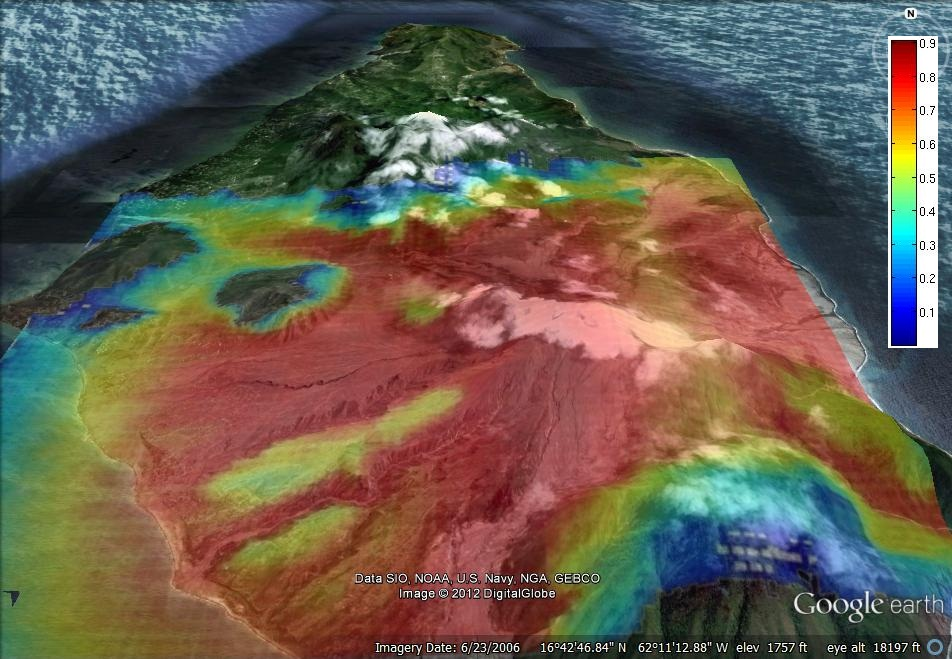
\includegraphics{new_map_colorbar.jpg}}%
\caption {Figure shows the probabilistic hazard map for the island of Montserrat in the Caribbean for flow exceeding 0.2m of depth.} \label{map2}
\end{center}
\end{figure}

The resulting 2048 pileheight records 
were merged using python
scripts and loaded on the Netezza server for downsampling and neighbor searching. The details of some of the tables generated are already provided
in Table 1. The dimensions associated with the random
variables being vastly different and having very different scales, were all mapped to the same scale of 0 to 1. Matrix operations being
expensive, it was essential to keep their sizes small. Thus a limit on the number of neighbors had to be
enforced in addition to a limit on the euclidean distance.

The computational details of the hazard map shown in figure \ref{maps}are enumerated below.
\begin{enumerate}
{
\item The Hazard map was generated using the our computational model comprising of the Netezza server and
504 processors on the high performance cluster.
\item Neighbor search, downsampling and few other operations were performed on Netezza in 30 minutes. The radius of neighborhood was fixed at 
0.3 for parametric dimensions
(scaled) and 200 metres for spatial dimensions. Furthermore, each sample point could have at most 500 neighbors and this
information was stored in the table $\small{PROXIMITY}$.
\item 504 processors functioning as 18 independent groups were responsible for emulator construction and the evaluation of mean and variance
using Bayes Linear model. Each group had 1 I/O processor and at most 27 compute processors.
\item During 8 hours 47 minutes of wall time on the cluster, approximately 4 million covariance matrices of size 300x300 were computed
through an iterative process and mean and variance was computed for approximately $10^{10}$ resample points.
\item In that time more than 1.5 TB of data was transferred over the network to Netezza server over 18 different pipes. 
This data was stored on 18 different tables occupying a little more than a total of 50 billion rows.
\item The final step which required scanning billions or rows of data to evaluate the barycentric weights and aggregate the results
was also performed on the Netezza server and took 2.5 hours of time.
\item The entire operation completed in little under 12 hours of time.\\
}
\end{enumerate}

%%%%%%%%%%%%%%%%%%%%%%%%%%%%%%%% END  OF COMMENTS  %%%%%%%%%%%%%%%%%%%%%%%%%%%%%%%%%%%%%%%%%%%%%%%%%%%%%%%%%%%%%%%%%%

\section{Results}
We put both computing models was put to test with the task of creating the hazard map for the volcano on Montserrat island. 
2048 sets of input parameters were generated using Latin Hypercube sampling and Titan2D simulations of these inputs were performed. 
The probabilistic hazard map shown on the left in figure \ref{map2} was generated, 
%with the same input parameters and with above modifications
%incorporated in the code, 
in 6 hours time using Netezza based workflow.
Downsampling and neighbor search operations were performed in under 30 minutes of time.
The computation time on the cluster was
reduced to a little more than 2.5 hours using 512 processors on 43 nodes of 12 cores each and by keeping 16 connections open between Netezza
and the cluster. The 512 processors were divided into 16 groups with each group having 1 I/O processor and at most 32 compute processors.
A maximum limit of 120 was enforced on the size of the covariance matrices.
Also the radius of search was reduced from 100 metres for spatial dimensions and from 0.2 for parametric dimensions(scaled).
The final aggregation was completed in 2.5 hours, and was performed entirely on Netezza server.\\

The probabilistic map on the right in figure \ref{maps} 
was generated with Hadoop based model. The  neighbor search operations were completed in 20 minutes of 
wall time. Emulator construction was performed individually by separately dispatching tasks on the cluster. This was completed in approximately 5
hours of time and resulted in 800GB of output data. Hadoop was extensively used for aggregation of results through two separate reduce processes.
200 reduce tasks were spawned over 30 nodes (1 master and 29 slave nodes) for the first reduce operation and the computations ended successfully
in approximately 8 hours of wall time reducing 800GB of data to 190GB of output. The second reduce operation was completed with 100 reduce tasks 
spread over on 20 nodes (1 master and 19 slave) in 1.5 hours of time.

%%%%%%%%%%%%%%%%%%%%%%%%%%%%%%%%%%%%%%%%%%%% BEGIN COMMENTS      %%%%%%%%%%%%%%%%%%%%%%%%%%%%

\subsection{Performance Optimization}
The Hazard map in figure \ref{map1}(b)  was generated in 12 hours of wall time. A significant portion of this time was spent on the
cluster and in moving the data across, posing a problem which attracted our attention. To understand the reason for long computation time,
it must be noted that every successful load session must be followed by the "generate statistics" command on the table which is loaded.
A load session is said to be complete when the pipe that is opened for writing is closed.
A single write session on the other hand involves writing all the data accumulated with I/O processor (for sending over to the server), to the
open pipe, clearing space in the memory for more data. We were able to improve the performance and reduce the time of computation on the cluster
by making communications between the I/O processors and the server less frequent and by introducing minor changes to the design.\\

\textbf{More write sessions per load session:}
Having more write sessions and few load sessions
reduced the number requests from the I/O processors to Netezza database to ``generate statistics" on the tables 
 resulting in less overall latency.

\textbf{Single processor handles ``generate statistics":}
The I/O processors were relieved of the job of prompting the server to ''generate statistics" on the tables, which was delegated to
the single processor that also assigns the sample numbers to the I/O processors. This was possible because the load sessions were now less frequent.
Fewer interactions between I/O processors and Netezza server, also led to I/O processors dispatching jobs to the compute processors with less
interruptions.\\

\textbf{Avoid simultaneous aggregation and loading:}
Simultaneous loading and aggregation of data on the server was to found to impede the performance. 
By avoiding this and instead scheduling the aggregation process for the end we were able to speed up the process.

\textbf{Column distribution:}
Prior distribution of tables based on ``columns" of interest ensures appropriate data slicing at the time of loading 
significantly reducing query response time.

\textbf{Writing in blocks:}
For I/O intensive operations such as ours writing in blocks led to notable reduction in time.
For our purpose we found 1KB sized blocks to produce the best results. 

Implementing these features resulted in cutting the total time taken by over 50\%.

\begin{figure}[H]
\begin{center}
\resizebox*{8cm}{!}{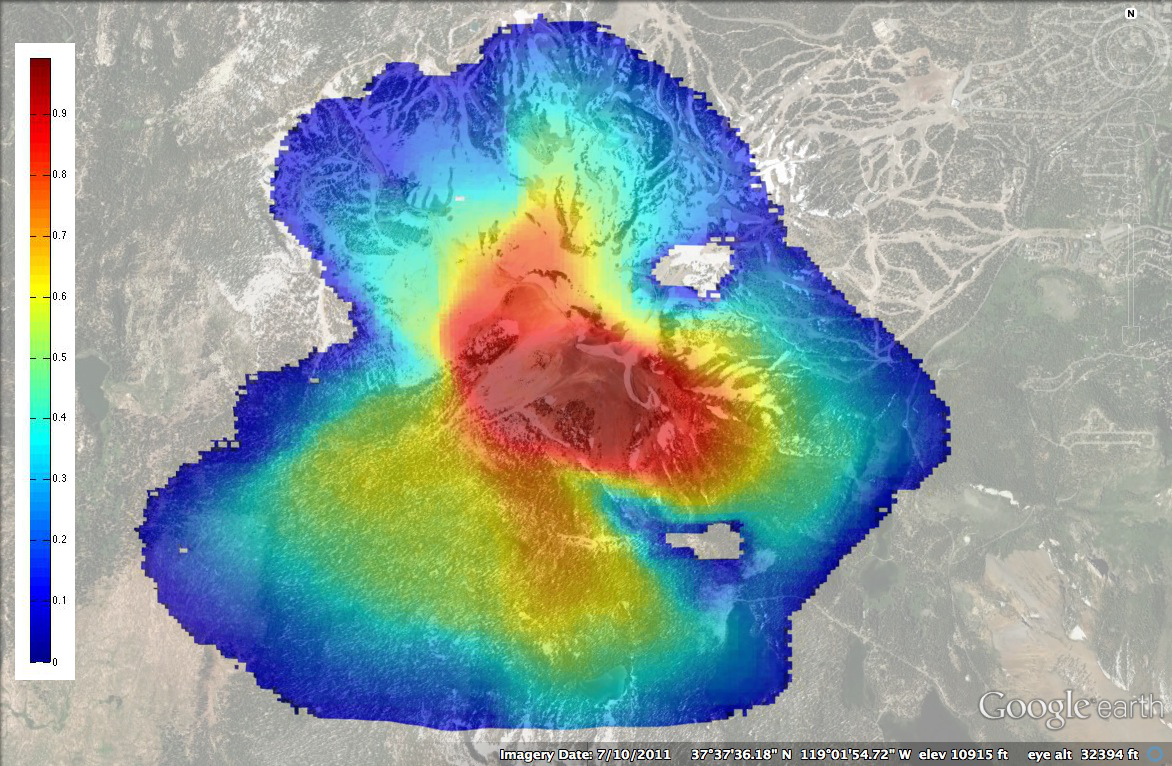
\includegraphics{mammoth.jpg}}%
\caption{\label{fig2} Figure shows the probabilistic hazard map (right) of the region around "Mammoth" volcano, 
for flow exceeding 0.2m of depth using 1024 samples generated with the above computing model.
}
\label{map2}
\end{center}
\end{figure}
%%%%%%%%%%%%%%%%%%%%%% END  OF COMMENTS  %%%%%%%%%%%%%%%%%%%%%%%%%%%%%%%%%%%%%%%%%%%%%%%%%%%%%%%%%%%%%%%%%%



\section{CONCLUSION}
%The primary contribution of 
Through this paper is we aim to address the simultaneous computational and data challenges in a Uncertainty quantification process
%using a combination of algorithmic (localization and parallelization) and hardware approaches.
through two different approaches - one hardware based and other using a more popular software tool on the traditional cluster.
%An integrated workflow was successfully architected, 
We successfully architected and implemented two functional workflows for the application of generating hazard maps for geophysical flows.
Netezza based workflow offered a faster implementation for a moderate sized data such as ours in comparison to Hadoop based workflow.
Data mining tasks required minimal work
and its ability to perform fast analytics provided quick insight about the data. On the other hand, Netezza is an expensive hardware, with its
SPUs (Snippet Processing Units) prone to wearing out. Integrating Netezza with the cluster presented numerous hurdles and the
resulting implementation was not fault tolerant. Furthermore, restriction on the  number of 'working' ports on Netezza makes the workflow less
scalable. Hadoop in contrast is a much cheaper alternative, offering reliable and robust job scheduler and fault tolerance. It made our
implementation of the workflow programatically easy and obviated the need to move data from the cluster. It is also more easily scalable.
However, modeling, a compute intensive
task, such as emulator construction, as a mapper posed a severe problem. Using Hadoop API for tasks deficient in input data but requiring more cpu
cycles clearly suggested that it can't be used as an alternative job scheduler for compute intensive tasks.

A number of fundamental changes in the design of hazard map generation were introduced and were largely possible through the use of
Netezza server. 




With Netezza's data mining capability, tessellation based covariance localization \cite{keith,ramona} was completely replaced with a more  reliable distance based search for neighbors.
This not only leads to a more precise control of the region of neighborhood but also makes it more feasible to extend the problem to higher
dimensions. In addition search distance for each dimension can be separately incorporated making this model even more versatile.
The tessellation based method is firmly dependent on the manner in which spatial points are downsized making $\it{downsampling}$ a cornerstone in 
the process emulator construction. The workflow proposed in this paper attributes less importance to $\it{downsampling}$ 
and offers more flexibility than the previous approach.\\

It was also comparatively easier to work on a combination of Netezza server and the high performance cluster. The codes were more concise and
amenable to changes. Most importantly, information was communicated in a more elegant fashion, with very little need for
file handling. Data was pre-dominantly transferred over the network obviating the need to read and write large number of ASCII files.
Finally, this model is easily extended to a wide range of problems with 
the similar challenges of massive data movement and complex computations.


% An example of a floating figure using the graphicx package.
% Note that \label must occur AFTER (or within) \caption.
% For figures, \caption should occur after the \includegraphics.
% Note that IEEEtran v1.7 and later has special internal code that
% is designed to preserve the operation of \label within \caption
% even when the captionsoff option is in effect. However, because
% of issues like this, it may be the safest practice to put all your
% \label just after \caption rather than within \caption{}.
%
% Reminder: the "draftcls" or "draftclsnofoot", not "draft", class
% option should be used if it is desired that the figures are to be
% displayed while in draft mode.
%
%\begin{figure}[!t]
%\centering
%\includegraphics[width=2.5in]{myfigure}
% where an .eps filename suffix will be assumed under latex, 
% and a .pdf suffix will be assumed for pdflatex; or what has been declared
% via \DeclareGraphicsExtensions.
%\caption{Simulation Results}
%\label{fig_sim}
%\end{figure}

% Note that IEEE typically puts floats only at the top, even when this
% results in a large percentage of a column being occupied by floats.


% An example of a double column floating figure using two subfigures.
% (The subfig.sty package must be loaded for this to work.)
% The subfigure \label commands are set within each subfloat command, the
% \label for the overall figure must come after \caption.
% \hfil must be used as a separator to get equal spacing.
% The subfigure.sty package works much the same way, except \subfigure is
% used instead of \subfloat.
%
%\begin{figure*}[!t]
%\centerline{\subfloat[Case I]\includegraphics[width=2.5in]{subfigcase1}%
%\label{fig_first_case}}
%\hfil
%\subfloat[Case II]{\includegraphics[width=2.5in]{subfigcase2}%
%\label{fig_second_case}}}
%\caption{Simulation results}
%\label{fig_sim}
%\end{figure*}
%
% Note that often IEEE papers with subfigures do not employ subfigure
% captions (using the optional argument to \subfloat), but instead will
% reference/describe all of them (a), (b), etc., within the main caption.


% An example of a floating table. Note that, for IEEE style tables, the 
% \caption command should come BEFORE the table. Table text will default to
% \footnotesize as IEEE normally uses this smaller font for tables.
% The \label must come after \caption as always.
%
%\begin{table}[!t]
%% increase table row spacing, adjust to taste
%\renewcommand{\arraystretch}{1.3}
% if using array.sty, it might be a good idea to tweak the value of
% \extrarowheight as needed to properly center the text within the cells
%\caption{An Example of a Table}
%\label{table_example}
%\centering
%% Some packages, such as MDW tools, offer better commands for making tables
%% than the plain LaTeX2e tabular which is used here.
%\begin{tabular}{|c||c|}
%\hline
%One & Two\\
%\hline
%Three & Four\\
%\hline
%\end{tabular}
%\end{table}


% Note that IEEE does not put floats in the very first column - or typically
% anywhere on the first page for that matter. Also, in-text middle ("here")
% positioning is not used. Most IEEE journals/conferences use top floats
% exclusively. Note that, LaTeX2e, unlike IEEE journals/conferences, places
% footnotes above bottom floats. This can be corrected via the \fnbelowfloat
% command of the stfloats package.



\section{Conclusion}
The conclusion goes here. this is more of the conclusion

% conference papers do not normally have an appendix


% use section* for acknowledgement
\section*{Acknowledgment}


The authors would like to thank...
more thanks here


% trigger a \newpage just before the given reference
% number - used to balance the columns on the last page
% adjust value as needed - may need to be readjusted if
% the document is modified later
%\IEEEtriggeratref{8}
% The "triggered" command can be changed if desired:
%\IEEEtriggercmd{\enlargethispage{-5in}}

% references section

% can use a bibliography generated by BibTeX as a .bbl file
% BibTeX documentation can be easily obtained at:
% http://www.ctan.org/tex-archive/biblio/bibtex/contrib/doc/
% The IEEEtran BibTeX style support page is at:
% http://www.michaelshell.org/tex/ieeetran/bibtex/
\bibliographystyle{IEEEtran}
\bibliography{list}
% argument is your BibTeX string definitions and bibliography database(s)
%\bibliography{IEEEabrv,../bib/paper}
%
% <OR> manually copy in the resultant .bbl file
% set second argument of \begin to the number of references
% (used to reserve space for the reference number labels box)
%\begin{thebibliography}{1}
%
%\bibitem{IEEEhowto:kopka}
%H.~Kopka and P.~W. Daly, \emph{A Guide to \LaTeX}, 3rd~ed.\hskip 1em plus
%  0.5em minus 0.4em\relax Harlow, England: Addison-Wesley, 1999.
%
%\end{thebibliography}




% that's all folks
\end{document}


